\documentclass[12pt]{basque-book}
\usepackage[a4paper]{geometry}
\usepackage[myheadings]{fullpage}
\usepackage{fancyhdr}
\usepackage{lastpage}
\usepackage{graphicx, wrapfig, subcaption, setspace, booktabs}
\usepackage[T1]{fontenc}
\usepackage[font=small, labelfont=bf]{caption}
\usepackage{fourier}
\usepackage[protrusion=true, expansion=true]{microtype}
\usepackage[basque]{babel}
\usepackage{sectsty}
\usepackage{url, lipsum}
\usepackage{graphicx}
\usepackage[utf8]{inputenc}
\usepackage{courier}
\usepackage{ulem}
\usepackage{spverbatim}
\usepackage{multirow} 
\usepackage{color}
\usepackage{graphicx}
\usepackage{epsfig}
\usepackage{multirow}
\usepackage{colortbl}
\usepackage{xcolor}
\usepackage{float}
\usepackage{fancyvrb}
\usepackage{bera}
\usepackage{adjustbox}
\usepackage{amsmath}
\usepackage{hyperref}
\usepackage[hyphenbreaks]{breakurl}


\usepackage{listings} 


\newcommand{\HRule}[1]{\rule{\linewidth}{#1}}
\onehalfspacing
\setcounter{tocdepth}{5}
\setcounter{secnumdepth}{5}

%-------------------------------------------------------------------------------
%Orrialde oina eta orrialde goiburua
%-------------------------------------------------------------------------------
\pagestyle{fancy}
\fancyhf{}
\setlength\headheight{15pt}
\fancyhead[R]{\MakeUppercase{matematika diskretua}}
\fancyfoot[C]{\thepage}
%-------------------------------------------------------------------------------
% Tituluaren orria
%-------------------------------------------------------------------------------

\begin{document}

\title{ \textbf{Matematika Diskretua\\ RSA Kriptografia Txostena} }

\author{Xabier Garrote}

\date{\today a}


\maketitle
\newpage
\tableofcontents
\newpage


%--------------------------------------------------------------------% Documentuaren atalak ezberdinak hemendik aurrera ---------------------------------------------------------------------
\chapter{Sarrera}
Euskaltzaindiaren arabera \textbf{kriptografia} "\textit{Ezkutuko kodeen bidez idazteko modua}" da. Hau da, mezu baten edukia igorleak eta hartzaileak \textbf{bakarrik} irakurtzeko kriptografia erabiltzen da.
\\\\
Igorleak mezua bidaltzean zifratu egiten du. Hartzaileak mezua jasotakoan, deszifratu egiten du irakurri ahal izateko. 
\\
Historian zehar hainbat kriptografia sistema ezberdin erabili dira.

\section{Antzinako kriptografia sistemak}
\subsection{Espartanoek K.a. V mendean} Mezuak ohial baten gainean idazten zituzten. Mezua zifratzeko ohiala loditasun jakin bateko makil baten gainean inguratzen zuten. Ondoren, mezua idazten zuten eta hartzaileari bidali. Hartzaileak mezua jasotzean igorlearen loditasun bereko makil batez baliatuz bertako edukia irakur zezakeen.


\newpage


\subsection{Polybiosen zifratze-sistema}  K.a II mendean sortutakoa. 
\begin{center}
    \begin{tabular}{ c |c |c| c| c| c| }
        & \textbf{A}  & \textbf{B} & \textbf{C} & \textbf{D} & \textbf{E} \\
         \hline
        \textbf{A}  &a  & b & c & d & e \\ 
        \hline
        \textbf{B}  &f  & g & h & i/j & k\\  
        \hline
        \textbf{C}  & l  & m & n & o & p \\
        \hline
        \textbf{D}  & q  & r & s & t & u\\
        \hline
        \textbf{E}  & v  & w & x & y & z
    \end{tabular}
\end{center}

Letra bakoitza matrizean duen kordenadengatik ordezkatzen da. Adibidez, \textbf{a} letra \textbf{AA} izango litzateke, \textbf{q} letra \textbf{DA} eta abar.

Zifratze sistema hau 25 karakterentzako pentsatuta dago, beraz, guk erabiltzen dugun alfabetora egokitzeko i eta j lauki berean jarri behar dira.

Mezua deszifratu ostean bi aukera geldituko dira i izatea edo j izatea baina kontextua eta hitzaren esker ez da dudarik egoten.

Adibidez: \textbf{Wikipedia}
\begin{itemize}
    \item Zifratzea:
    \begin{center}
        \begin{tabular}{c|c|c|c|c|c|c|c|c|c|}
             W & i & k & i & p & e & d & i & a\\ 
             \hline
             EB & BD & BE & BD & CE & AE & AD & BD & AA
        \end{tabular}
    \end{center}
    \begin{center}
        Hitz zifratua:\textbf{EB BD BE BD CE AE AD BD AA}
    \end{center}
    \item Deszifratzea:
    \begin{center}
        \begin{tabular}{c|c|c|c|c|c|c|c|c|c|}
            EB & BD & BE & BD & CE & AE & AD & BD & AA\\
            \hline
            W & i/j & k & i/j & p & e & d & i/j & a\\ 
        \end{tabular}
        \\
    \end{center}
    \begin{center}
         Hitz deszifratua:\textbf{Wikipedia}
    \end{center}
\end{itemize}


\subsection{Cesarren zifratua} 
Erromatarrek orain dela 2000 urte asmatutakoa.
Mezuak sekretu mantentzeko, jatorrizko mezuko letra bakoitza alfabetoan hiru posizio aurrerago zegoen letrarengatik ordezkatzen zuten.

Horrela, hartzaileak jasotako mezuko letra bakoitza alfabetoan hiru posizio atzerago zegoen letrarengatik ordezkatu behar zuen. Ordezkatu ostean, jatorrizko mezua irakurtzeko gai zen.

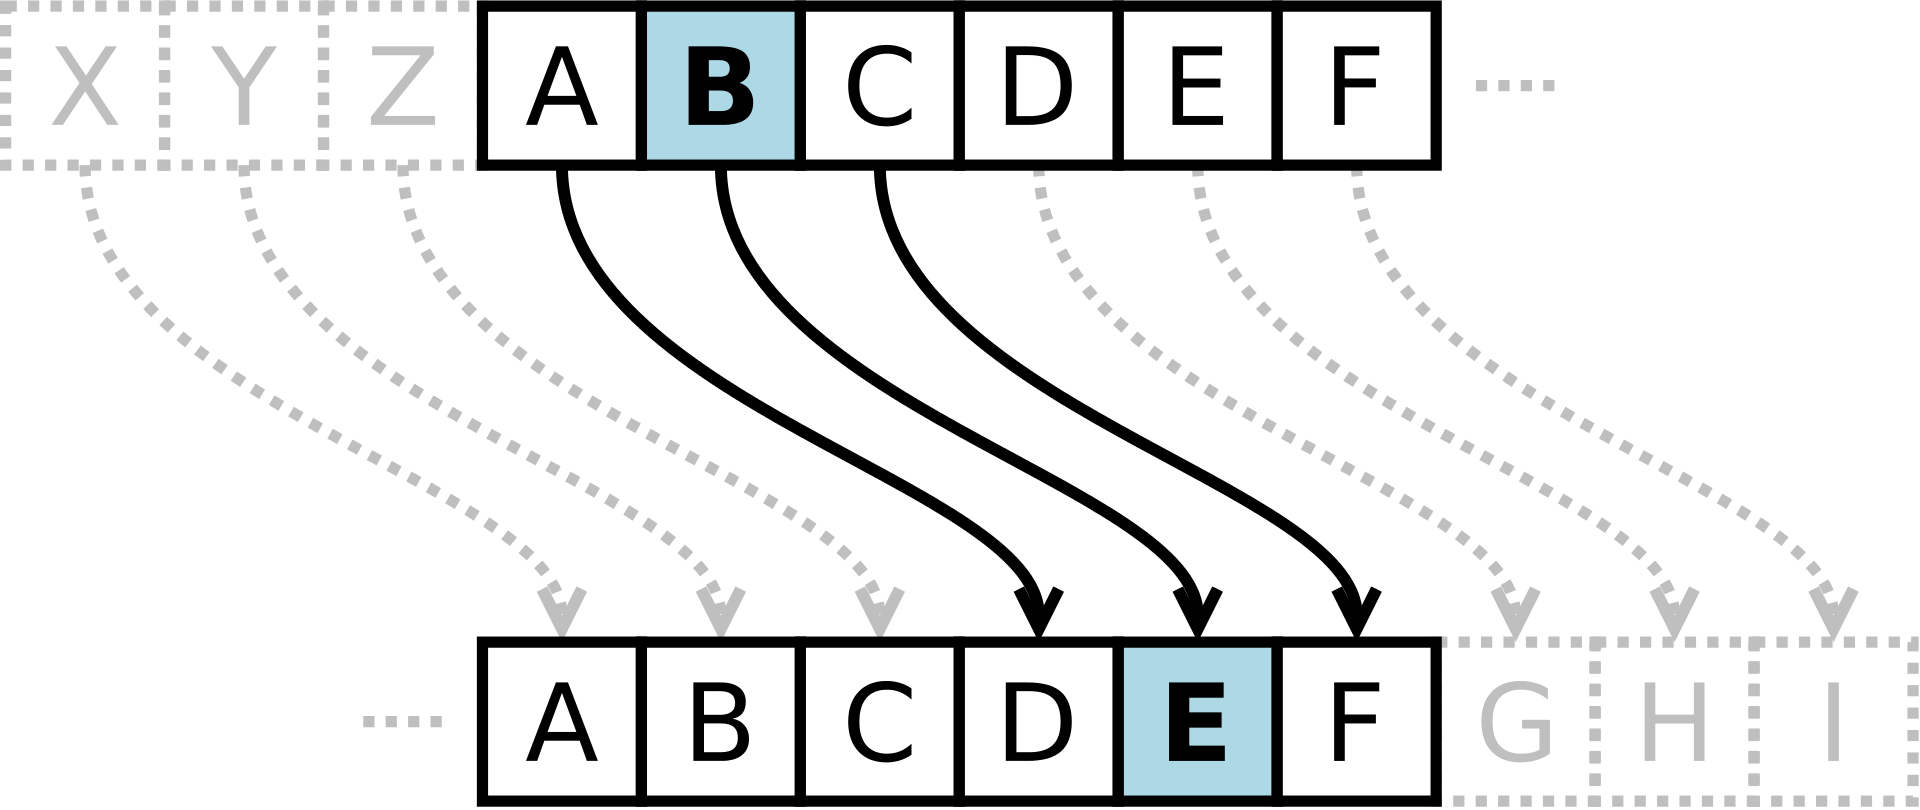
\includegraphics[scale=0.1]{Zesar_zifratu.png}

\begin{itemize}
    \item \textbf{Jatorrizko alfabetoa}: abcdefghijklmnñopqrstuvwxyz
    \item \textbf{Alfabeto zifratua}: defghijklmnñopqrstuvwxyzabc
\end{itemize}

\section{Bigarren gerra mundiala}

\subsection{Alan Turing eta Enigma makina}
Mundua bigarren gerra mundialean murgilduta zegoela. Naziek enigma makina erabiltzen zuten beraien mezuak zifratu eta deszifratzeko.
\\\\
Naziek segurua zela uste zuten Alan Turing agertu arte. Britania Handiak, Enigma makina baten replika lortu zuen. Ondoren, Alan Turing eta garaiko beste hainbat matematikari Britania Hanidan bildu ziren. Hauek, buru belarri aritu ziren makina ikertzen eta honi nola aurre egin pentsatzen.
\\\\
Enigmak tekla bat sakatzen zen heinean 3 errotorez baliatuz beste letra batengatik ordezkatzen zen. Guztira 10.000 billoi konfigurazio posible ezberdin zeuden. Mezuak deszifratzeko, beste enigma makina bat eta honen hasierako errotoreen konfigurazioa jakin behar zen. Naziek egunero errotoren hasierako konfigurazioa aldatzen zuten.
\\\\
Hasiera batean, erabilitako teknikak papera eta arkatzen bidezkoak ziren. Baina Alan Turing-ek makina bati aurre egiteko beste makina bat sortu zuen \textbf{Bombe}.
\\\\
\textbf{Bombe makinak} bilaketa sistematiko bat egiten zuen kontsiderazio logiko batzuekin enigmaren hasierako errotoreen konfigurazioa lortzeko.

\section{Bigarren gerra mundialaren ondoren}
\subsection{RSA zifratze algoritmoa}
RSA 1977 urtean Ronald Rivest, Adi Shamir eta Leonard Adlemanek sortu zuten kriptografia-sistema edo zifratze-sistema da.
\\\\
Zenbaki teorian oinarritutako zifratze sistema bat da. Non pauso batzuk jarraituz, gako publiko eta pribatua kalkulatzen diren.
\begin{itemize}
    \item \textbf{Gako publikoa:} Besteek zuri mezuak idaztean zifratzeko erabili behar duten gakoa.
    (hauek publiko egin behar dira besteek ezagun dezaten)
    \item \textbf{Gako pribatua:} Besteek zuri idatzitako mezuak deszifratzeko erabili behar duzun gakoa.(hau EZ da inoiz publiko egin behar)
\end{itemize}
Hona hemen adibide bat:
\begin{itemize}
    \item \textbf{Mikelen gakoak n =  143 , r =  7 , s = 103}
    \item Mikel eta Jon-en arteko elkarrizteka:
    \begin{itemize}
    \item Mikelen gako publikoa:
    \textbf{n =  143 , r =  7} dira
    \item Jonek mezua zifratuko du mikelen gako publikoa erabiliz:\newline
    \textbf{65 18 59 98  4 59 38 39 33 71 24}
    \item Mikelek bere gako pribatua erabiliz mezua deszifratuko du:\newline
    \textbf{Apa lagun;)}
    \end{itemize}
\end{itemize}
RSA-ren segurtasuna zenbaki handien faktorizatzeko probleman dago. Gaur egun, ez dago algoritmo eraginkorrik problema honi aurre egiteko. Beraz, gaur egun zifratze-sistema on bat da RSA gako handiak aukeratzen badira.
\begin{itemize}
    \item Goiko abidideko \textbf{n=143} faktorizatzen saiatzen bagara:
    \begin{verbatim}
    > n<-143
    > b<-primeFactors(n)   #Ordenagailua gakoak kalkulatzeko kapaza da
    > RSA_gakoak(b[1],b[2]) #Irteera bera dute gako pribatua deskubrituta
    n =  143 , r =  7 , s = 103
    \end{verbatim}
    \newpage
    \item Gako handiak aukeratuz: \textbf{n=773977589210346518720862 , r =  2634758697353 , s = 391747678355017485524800}
    \item\textbf{n=773977589210346518720862} faktorizatzen saiatzen bagara:
    \begin{verbatim}
        > primeFactors(773977589210346518720862)
        [1] NA
        Warning message:
        In primeFactors(7.73977589210347e+23) :
          Argument 'n' too big: use 'gmp::factorize()' for this.
    \end{verbatim}
\end{itemize}
Gako seguruak aurikitu ditugu:\newline
\textbf{n=773977589210346518720862 , r =  2634758697353\newline
, s = 391747678355017485524800}
\\\\
RSA-algoritmoa ikusi dugun bezala gaur egun segurua da eta ondorioz hainbat tokitan erabiltzen da esate baterako Whatsapp,DNI txarteletan eta TLS interneteko konexioen zertifikatuetan.
\\\\
Historian zehar ikusi dugun bezala, zifratze algoritmoak gero eta konplexuagoak dira. Algorimo zaharrak baztertuta gelditzen ziren heinean, seguruak ez zirelako algorimto konplexuagoak agertzen ziren.
\\\\
Gaurko egun RSA algoritmoaz aparte beste hainbat daude AES eta 3DES bezalakoak.
\\\\
\textbf{Baina, noiz arte jarraituko dute algoritmo hauek seguruak izaten??}


\chapter{Inplementatutako funtzioen kodea}
\section{zkh 1.bertsioa}
\begin{verbatim}
    # Bi zenbaki oso emanik, a eta b, zatitzaile komunetako handiena 
    # kalkulatuko duen funtzioaren inplementazioa Euklidesen algoritmoan
    # oinarrituz:
    zkh <- function(a,b){ 
        c<-a;
        d<-b;
        while (d != 0) {
            r=mod(c,d);
            c=d;
            d=r;
        }
        return(c)  
    }
\end{verbatim}

\newpage
\subsection{Deiak funtzioari}
\begin{verbatim}
    > zkh(2689,4001)
    [1] 1
    > zkh(1369,2597)
    [1] 1
    > zkh(3.2,4)
    Error in mod(c, d) : 
    Arguments 'n', 'm' must be integers or vectors of integers. 
    > zkh("a","b")
     Error in mod(c, d) : is.numeric(n) is not TRUE 
\end{verbatim}

\newpage

\section{zkh 2.bertsioa}
\begin{verbatim}
    # Parametro moduan jasotako a,b Euklidesen algoritmoan oinarrituz
    # zatitzaile komunetako handiena itzuliko du
    # Parametro moduan zenbaki errealak pasaz gero, errore
    # mezua erakutsiz, karaktereak pasaz gero, baita.
    zkh <- function(a,b){ 
        if(is.character(a)==FALSE & is.character(b)==FALSE){
            c=abs(a)
            d=abs(b)
            if(isNatural(c)&isNatural(d)){
                c<-a;
                d<-b;
                while (d != 0) {
                    r=mod(c,d);
                    c=d;
                    d=r;
                }
                return(c)
            }
            else{
                print('a eta b parametroak zenbaki osoak izan behar dute.')
            }
        }
        else{  
            print('a eta b ezin dira karaktereak izan.')
        }
    }
\end{verbatim}

\newpage

\subsection{Deiak funtzioari}
\begin{verbatim}
    > zkh(231,1820)
    [1] 7
    > zkh(1369,2597)
    [1] 1
    > zkh(3.2,4)
    [1] "a eta b parametroak zenbaki osoak izan behar dute." 
    > zkh(5,'b')
    [1] "a eta b ezin dira karaktereak izan."
\end{verbatim}

\newpage
\section{lehen\_erlatibo\_txiki}
\begin{verbatim}
    # Parametro moduan funtzioari pasatako m-rekin lehen erlatiboa 
    # den zenbaki oso positiborik txikiena itzuliko du
    # RSA_gakoak funtzioa inplementatzeko erabiliko dugu
    lehen_erlatibo_txiki <- function(m){
        zk = 2
        while (GCD(m, zk) != 1){
            zk = zk + 1;
        }
        return(zk);
    }
\end{verbatim}

\subsection{Deiak funtzioari}
\begin{verbatim}
    > lehen_erlatibo_txiki(13797)
    [1] 2
    > # 2
    > lehen_erlatibo_txiki(16974)
    [1] 5
    > # 5
    > lehen_erlatibo_txiki(56970)
    [1] 7
    > # 7
    > lehen_erlatibo_txiki(1000000000000000)
    [1] 3
\end{verbatim}
    
\newpage

\section{RSA\_gakoak}
\begin{verbatim}
    # Bi zenbaki lehen emanik, p eta q, n, r eta s kalkulatuko 
    # ditu, eta irteera estandarretik inprimatu. r txikia kalkulatuko
    # da.
    RSA_gakoak <- function(p,q){
        n = p * q;
        m = (p - 1) * (q - 1);
        r = lehen_erlatibo_txiki(m); #goian azaldutako funtzioa
        s = modinv(r, m);
        cat("n = ", n, ", r = ", r, ", s = ", s); 
    }
\end{verbatim}
\subsection{Deiak funtzioari}
\begin{verbatim}
    > RSA_gakoak(5,17)
    n =  85 , r =  3 , s =  43
    > RSA_gakoak(17,23)
    n =  391 , r =  3 , s =  235
    > RSA_gakoak(97,101)
    n =  9797 , r =  7 , s =  2743
    > RSA_gakoak(307,397)
    n =  121879 , r =  5 , s =  96941
\end{verbatim}

\newpage

\section{kodetu}
\begin{verbatim}
    # Parametro moduan txt karaktere string-a jaso eta dagozkion  
    # ASCII kodeak itzultzen ditu.
    kodetu <- function(txt){
        return(strtoi(charToRaw(txt), 16L));
    }
\end{verbatim}

\subsection{Deiak funtzioari}
\begin{verbatim}
    # Ondoren, deskodetu funtzioarekin konprobatuko dugu  
    # ondo kodetu direla
    > testu1<-"kaixo"
    > kodebektore1<-kodetu(testu1)
    > kodebektore1
    [1] 107  97 105 120 111
    > testu2<-"KAIXO"
    > kodebektore2<-kodetu(testu2)
    > kodebektore2
    [1] 75 65 73 88 79
    > testu3<-"Zer moduz?"
    > kodebektore3<-kodetu(testu3)
    > kodebektore3
     [1]  90 101 114  32 109 111 100 117 122  63
\end{verbatim}

\newpage

\section{deskodetu}
\begin{verbatim}
    # Parametro moduan ASCII kodeak jaso eta dagokion txt karaktere 
    # string-a itzultzen duen funtzioa.
    deskodetu <- function(kodetxt){
        return(rawToChar(as.raw(kodetxt)));
    }   
\end{verbatim}

\subsection{Deiak Funtzioari}
\begin{verbatim}
    # Kodetu funtzioarekin kodetutatko bektoreak 
    # deskodetuko ditugu
    > txt1<-deskodetu(kodebektore1)
    > txt1
    [1] "kaixo"
    > txt2<-deskodetu(kodebektore2)
    > txt2
    [1] "KAIXO"
    > txt3<-deskodetu(kodebektore3)
    > txt3
    [1] "Zer moduz?"
\end{verbatim}

\newpage

\section{zifratu}
\begin{verbatim}
    # Parametro moduan ASCII kodeez osatutako bektore bat jaso eta 
    # dagokion bektore zifratua itzuliko du
    zifratu <- function(kodebektorea,r,n){
        luzeera = length(kodebektorea);
        for (i in 1:luzeera)
        {
            kodebektorea[i] = modpower(kodebektorea[i], r, n);
        }
        return(kodebektorea);
    }
\end{verbatim}

\subsection{Deiak funtzioari}
\begin{verbatim}
    > # Erabiliko ditugun gakoak:
    > # n=9797, r=7, s=2743
    > n<-9797
    > r<-7
    > bektorezifratu1<-zifratu(kodebektore1,r,n)
    > bektorezifratu1
    [1] 2792 5432 4668 4973 7969
    > bektorezifratu2<-zifratu(kodebektore2,r,n)
    > bektorezifratu2
    [1] 7976 4764 2565 8540 4974
    > bektorezifratu3<-zifratu(kodebektore3,r,n)
    > bektorezifratu3
     [1]  375 2222 7721 3675  493 7969 6261 8564 4122 4604
\end{verbatim}

\newpage

\section{deszifratu}
\begin{verbatim}
    # Parametro moduan bektore zifratu bat jaso eta dagozkion 
    # ASCII kodeak itzuliko du
    deszifratu <- function(bektorezifratu,s,n){
        luzeera = length(bektorezifratu);
        for (i in 1:luzeera)
        {
            bektorezifratu[i] = modpower(bektorezifratu[i], s, n);
        }
      return(bektorezifratu);
    }
\end{verbatim}

\subsection{Deiak funtzioari}
\begin{verbatim}
    > # RSA_gakoak(97,101) zenbaki lehenetatik lortutako gakoekin:
    > # n=9797, r=7, s=2743
    > n<-9797
    > r<-7
    > s<-2743
    > testuberria<-"ea hau ondo doan..."
    > testuberri_zifratua <- zifratu(kodetu(testuberria),r,n)
    > testuberri_zifratua
     [1] 2222 5432 3675 1177 5432 8564 3675 7969 9305 6261
    [11] 7969 3675 6261 7969 5432 9305 3037 3037 3037
    > testuberri_errekuperatua <- deskodetu(deszifratu(testuberri_zifratua,s,n))
    > testuberri_errekuperatua
    [1] "ea hau ondo doan..."
\end{verbatim}


\chapter{Iritzi pertsonala}

Lehenengo eta behin, Matematika Diskretuan kriptografia buruz egindako laborategiak asko gustatu zaizkit. Alde batetik, oso interesgarriak iruditu zaizkit RSA zifratze algoritmoaren funtzionamendua ikasteko. Gainera, denbora ziztu bizian pasatzen zen. Bestetik, laborategi saio gehiago izatea nahiko nuke RSA aparte beste zifratze algoritmoren bat aztertzeko, esate baterako \href{https://eu.wikipedia.org/wiki/Advanced_Encryption_Standard}{\textbf{AES}} edo \href{https://eu.wikipedia.org/wiki/DES_Hirukoitza}{\textbf{3DES}}. Aldiz, badakit horretarako ikasketa plana aldatu beharko zela eta hori ez da gauza erraza.
\\\\
Bigarrenik, laborategi saioak ondoren RSA kriptografia txosten bat idatzi dugu. Txostena egiteko oso ondo moldatu nahiz. Izan ere,ikasle errepikatzailea nahiz eta latex lehengo urtetik ezagutzen nuen. Gauzak horrela, Latex-eko aginduekin ez dut problemarik izan eta informazio gehiena wikipedia, xlsemanal eta informatikaren buruzko blogetan aurkitu dut.
\\\\
Laburbilduz, kriptografia buruz egin dugun lan hau interesgarria iruditu zait eta gogoz burutu dut.

\begin{thebibliography}{}
%Bibliografia aurkibidean egoteko
\addcontentsline{toc}{chapter}{Bibliografia}
%%%%%%%%%%%%%%%%%%%%%%%%%
\bibitem{}\url{https://eu.wikipedia.org/wiki/Kriptografia}

\bibitem{}\url{https://unamcriptografia.wordpress.com/category/tecnicas-clasicas-de-cifrado/sustitucion/monoalfabetica/monogramica/polybios/}

\bibitem{}\url{https://encdesarrollo.wordpress.com/2012/10/09/cifrado-de-polybios/}

\bibitem{}\url{https://www.xlsemanal.com/conocer/tecnologia/20180614/historia-de-la-criptografia.html}

\bibitem{}\url{https://eu.wikipedia.org/wiki/Transport_Layer_Security}
\bibitem{}\url{https://eu.wikipedia.org/wiki/RSA}
\bibitem{}\url{https://eu.wikipedia.org/wiki/Enigma_(kriptografia)}
\bibitem{}\url{https://www.eldiario.es/turing/criptografia/Breve-historia-criptografia_0_261773822.html}


\end{thebibliography}
\end {document}